% Final project report, ACL format. Compile with pdflatex + bibtex (e.g. on Overleaf):
%   pdflatex report && bibtex report && pdflatex report && pdflatex report
\documentclass[11pt]{article}
\usepackage[preprint]{acl}
\usepackage{times}
\usepackage{latexsym}
\usepackage[T1]{fontenc}
\usepackage[utf8]{inputenc}
\usepackage{microtype}
\usepackage{inconsolata}
\usepackage{graphicx}
\usepackage{booktabs}
\usepackage{amsmath}
\usepackage{xcolor}

\newcommand{\dtbu}{BC$_{\mathrm{DTBU}}$}
\newcommand{\sigrw}{BC$_{\mathrm{SigRW}}$}

\title{Rebuilding and Attacking BSFR-SH: A Reproduction and Security Study\\
of a Blockchain-Based Ransomware Defence for Smart Healthcare}

\author{[Author names] \\
  Research in Information Security, course project \\
  [Institute] \\
  \texttt{[emails]}}

\begin{document}
\maketitle

\begin{abstract}
BSFR-SH \citep{wazid2023bsfrsh} proposes a ransomware defence for hospitals built on two private
blockchains: one stores encrypted backups, the other stores ransomware signatures collected by a
honeypot, and a machine-learning (ML) detector decides when to isolate a system and restore it.
The paper reports 98.98\% detection accuracy, throughput that grows with chain size, and
resistance to 51\% attacks. We rebuilt the whole framework from scratch in Python (both chains
under real pBFT consensus, all five algorithms, and the honeypot pipeline the paper leaves
undefined) and tested every claim. Our faithful rebuild reaches 94.4\%, on a test set where always
answering ``ransomware'' already scores 90\%. With 2 of its 4 servers malicious, the chain forks.
After the mid-semester evaluation we ran seven further experiments. They show that the rising
throughput is a one-off setup cost being averaged out, and that the detector mostly learns
\emph{which years} had ransomware: on years it has not seen it falls to 55\%, and retraining every
year does not help. Most importantly, the recovery step can be broken in two ways. A single
server holds the only key to every backup, and slow ransomware gets its encrypted files backed up
and later restored. We built and measured a fix for each: 2-of-4 key sharing and backup content
screening.
\end{abstract}

% =====================================================================================
\section{Introduction}

Ransomware encrypts a victim's files and demands payment for the key. Hospitals are attractive
targets because they cannot afford downtime: a locked patient record can delay treatment. The
usual defence is a good backup. A backup only helps, however, if the attacker cannot reach it,
cannot tamper with it, and has not already damaged the data inside it.

BSFR-SH \citep{wazid2023bsfrsh} addresses this with blockchain technology. Backups are encrypted
and written to a private blockchain whose blocks cannot be changed once committed
(\emph{immutability}). A honeypot, a decoy system meant to attract ransomware, collects attack
data onto a second blockchain, and an ML model trained on that data detects attacks. When an
attack is detected, the infected system is isolated and restored from the backup chain.

This report covers our course project on the paper, which had three goals, in order:
\begin{enumerate}
\setlength\itemsep{0pt}
\item \textbf{Reproduce} every claim the paper makes (its Table II and Figures 4--6).
\item \textbf{Re-evaluate} claims where the paper's method makes them look better than they are.
\item \textbf{Repair} design gaps we find, without breaking the reproduction.
\end{enumerate}
Section~\ref{sec:paper} summarises the paper and Section~\ref{sec:impl} our implementation.
Section~\ref{sec:mid} describes the work completed by the mid-semester evaluation, and
Section~\ref{sec:after} the seven experiments run after it to close the questions that work left
open. Section~\ref{sec:discussion} lists the paper's limitations and what it gets right.
Our own limitations are given in the Limitations section.

Our main contributions are:
(i) a complete, tested implementation of BSFR-SH;
(ii) evidence that its detection result rests on an unrealistic test set and a calendar
shortcut, and does not hold on future data;
(iii) a corrected security bound for its consensus layer, with a demonstrated fork;
(iv) an explanation of its throughput curve; and
(v) two attacks on its recovery step, each with a working fix.
Every number in this report was measured by us from a script with a fixed random seed and a saved
run log, unless it is labelled as the paper's.

% =====================================================================================
\section{The BSFR-SH Paper}
\label{sec:paper}

\begin{figure*}[t]
\centering
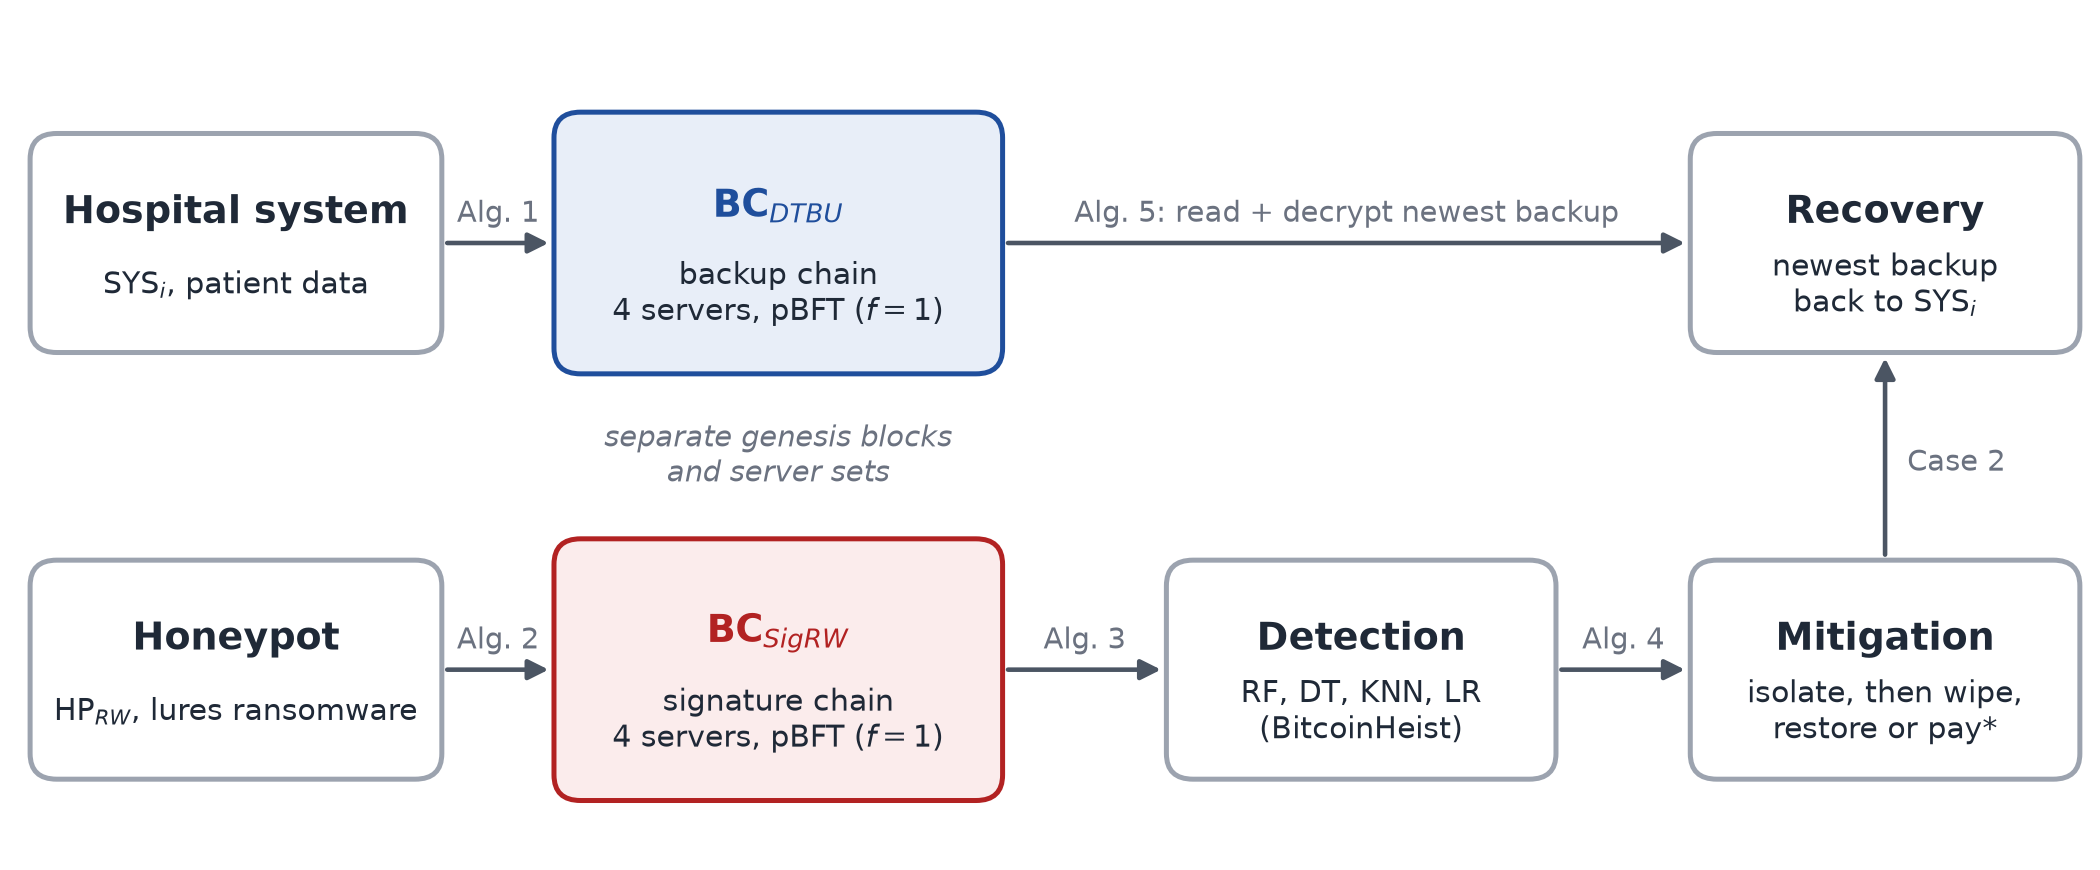
\includegraphics[width=0.92\textwidth]{figs/architecture.png}
\caption{BSFR-SH as specified by the paper and as we built it. Each chain has its own four cloud
servers running pBFT consensus, which tolerates one faulty server ($f=1$). *Case 3 (paying the
ransom) exists in our build only as a simulated decision that is always blocked.}
\label{fig:arch}
\end{figure*}

\paragraph{Architecture.}
Figure~\ref{fig:arch} shows the design. Two independent private blockchains are maintained by
cloud servers: \dtbu{} for data backups and \sigrw{} for ransomware signatures. Each is run by
four servers using \emph{practical Byzantine Fault Tolerance} (pBFT)
\citep{castro1999pbft}. A \emph{Byzantine} server is one that may lie or act maliciously; pBFT
stays correct while fewer than one third of servers are Byzantine ($n \geq 3f+1$), so four servers
tolerate one. Blocks are signed with ECDSA and transactions are encrypted to a cloud server's
public key.

\paragraph{Five algorithms.}
\textbf{Alg.~1} sends each hospital system's backup to a cloud server, which encrypts it and
commits it to \dtbu{}.
\textbf{Alg.~2} collects data from a honeypot, cleans it, extracts a signature and a feature
vector, and commits them to \sigrw{}.
\textbf{Alg.~3} trains four classifiers (random forest, decision tree, k-nearest neighbours (KNN)
and logistic regression) and runs detection.
\textbf{Alg.~4} isolates an infected system and then either removes the ransomware (Case~1),
formats the system and restores it (Case~2), or pays the ransom if it is cheaper than the data
(Case~3).
\textbf{Alg.~5} finds the system's newest backup on \dtbu{}, decrypts it and returns it.

\paragraph{Claims.}
Section~V of the paper argues informally that session keys stop replay, man-in-the-middle (MITM)
and impersonation attacks; that pBFT resists 51\% attacks; and that immutability stops tampering
and denial of service. Section~VII evaluates the detector on the BitcoinHeist dataset
\citep{akcora2020bitcoinheist}, which describes 2.9 million Bitcoin addresses, 1.42\% of them
used by ransomware. After resampling to 90\% ransomware and 10\% benign rows, the paper reports
\textbf{98.98\% accuracy and 0.990 F1} for its best model, the decision tree. It also reports
block-commit times for 5, 10 and 15 blocks of 100 transactions, with transactions per second
(TPS) rising from 161 to 263 on the backup chain (3.10, 4.17 and 5.71\,s) and from 115 to 222 on
the signature chain (4.36, 5.54 and 6.76\,s), measured with four Java processes on one laptop. It
compares its detector with four earlier ransomware detectors in its Table~II. The paper gives no
hyperparameters, no random seed, no split method and no transaction size, so none of its numbers
can be checked directly from the text.

% =====================================================================================
\section{Our Implementation}
\label{sec:impl}

We implemented everything from scratch in Python: SHA-256 Merkle trees, ECDSA signatures on the
secp256r1 curve, AES-256-GCM encryption, a mutual-authentication session protocol, our own pBFT
with leader change (view change), both chains with separate genesis blocks and server sets,
a honeypot sample generator and feature extractor, the four detectors, a mitigation state
machine, and recovery. The project has 1,884 automated tests, including tampered blocks, forged
signatures, equivocating Byzantine servers, replay and MITM attempts, and Sybil identities.

The paper leaves several parts unspecified. We filled each one deliberately and recorded the
reason:
\textbf{Hybrid encryption (ECIES).} An elliptic-curve public key cannot encrypt bulk data, so each
backup is encrypted with a fresh AES key, and that key is wrapped with the cloud server's public
key.
\textbf{Honeypot features.} The paper says signatures and features are ``generated'' and nothing
more. We defined 22 behavioural features in 7 groups (for example file-write entropy, rename rate
and shadow-copy deletions) and generate them statistically. No real malware is used.
\textbf{Preprocessing.} Alg.~2 says to ``remove the abnormalities''. Read literally on ransomware
data this removes the ransomware itself, since it is the abnormal class. We remove sensor faults
instead.
\textbf{Case~3.} Automatic ransom payment is implemented only as a decision that is logged and
always blocked. Nothing can pay.

\paragraph{How we measure.} \emph{Accuracy} is the share of rows labelled correctly. It is
misleading when one class dominates, so we also report \emph{precision} (of the rows flagged, how
many are ransomware), \emph{recall} (of the ransomware, how much is flagged), \emph{F1} (their
harmonic mean), \emph{balanced accuracy} (the average of the recall on each class, where any
constant answer scores 0.5), the \emph{false-positive rate} (benign rows wrongly flagged),
\emph{MCC} (a correlation between predictions and labels, 0 for guessing) and \emph{PR-AUC}.
Every result is compared with the score of a constant answer, the \emph{base rate}.

\paragraph{Reproducibility.} Every experiment is a script that takes a random seed and writes a run
log with its configuration and results; the post-mid-semester results are means over several seeds. Every
departure from the paper (50 in total) is recorded with its reason in a deviations log, and every
measured number is listed in a results log that this report draws from.

% =====================================================================================
\section{Work Until Mid-Semester}
\label{sec:mid}

\subsection{Detection: reproducing Table II}

\begin{table}[t]
\centering
\small
\begin{tabular}{@{}p{3.35cm}p{1.75cm}cc@{}}
\toprule
\textbf{Detector} & \textbf{Data} & \textbf{Acc.} & \textbf{F1} \\
\midrule
\multicolumn{4}{@{}l}{\emph{as reported in the paper's Table II}} \\
Almashhadani et al. & network traffic & .971 & .971 \\
Hwang et al. & dynamic logs & .973 & .973 \\
Sharmeen et al. & own corpus & .960 & .960 \\
Bae et al. & PE files & .987 & .987 \\
BSFR-SH (decision tree) & BitcoinHeist & \textbf{.990} & \textbf{.990} \\
\midrule
\multicolumn{4}{@{}l}{\emph{measured by us, same 90/10 BitcoinHeist sample}} \\
random forest & BitcoinHeist & .944 & .970 \\
decision tree & BitcoinHeist & .922 & .957 \\
logistic regression & BitcoinHeist & .900 & .948 \\
KNN & BitcoinHeist & .889 & .941 \\
always ``ransomware'' & BitcoinHeist & .900 & .947 \\
\bottomrule
\end{tabular}
\caption{Table II of the paper and our reproduction ($n=46{,}014$). The four earlier detectors were
evaluated on other datasets, so the paper's comparison is not like-for-like.}
\label{tab:table2}
\end{table}

\begin{table}[t]
\centering
\small
\begin{tabular}{@{}p{2.55cm}p{3.15cm}l@{}}
\toprule
\textbf{Paper claims} & \textbf{We measured} & \textbf{Verdict} \\
\midrule
98.98\% accuracy, 0.990 F1 & 94.42\% / 0.970 (RF, best of 4); always-``ransomware'' baseline 90.0\% / 0.947 & not reproduced \\
TPS grows with chain size & flat TPS once setup is excluded & see \S\ref{sec:a} \\
resists 51\% attacks & pBFT breaks at one third; 2 of 4 malicious servers fork the chain & wrong bound \\
session keys stop replay, MITM, impersonation & verified with Scyther & holds \\
\bottomrule
\end{tabular}
\caption{The paper's main claims against our mid-semester measurements.}
\label{tab:claims}
\end{table}

The paper's 90/10 resample has a hidden size limit. BitcoinHeist has only 41,413 ransomware rows,
so a sample that is 90\% ransomware can hold at most 46,014 rows: 1.6\% of the dataset the paper
describes. On this sample, a ``detector'' that always answers ransomware already scores 90.0\%
accuracy and 0.947 F1. This \emph{base rate} is the number every result must be compared with.

Following the paper's protocol, we dropped the \texttt{address} column (an identifier) and used a
\emph{grouped split}, so that each Bitcoin address appears only in training or only in test. Our
best model, random forest, reached \textbf{94.42\% accuracy and 0.970 F1}, 4.56 points below the
paper (Tables~\ref{tab:claims} and~\ref{tab:table2}). Table~\ref{tab:table2} also shows that the
four detectors the paper compares against were tested on different data (network traffic,
program logs, executable files), and that one of them clears the constant-answer baseline by only
0.013 F1. The paper's best model, the decision tree, reached 92.24\%. We then
tested eight possible explanations for the gap: keeping the address column, a random split,
splitting criterion, resampling strategy, seed variance, cross-validation, date features, and all
of these stacked. The best stacked combination reached 97.47\%, still 1.51 points short. The largest
single factor was oversampling ransomware rows under a random split, which puts copies of training
rows into the test set.

At the dataset's natural balance (1.42\% ransomware, all 2.9 million rows), accuracy is
meaningless (never predicting ransomware scores 98.6\%), so we report other metrics
(Table~\ref{tab:honest}). The random forest finds 29\% of ransomware addresses at 74\% precision
(MCC 0.457). Logistic regression flips behaviour completely: on the 90/10 sample it labels every
row ransomware, and at natural balance it labels every row benign. Full-scale KNN needed the
university's HPC cluster (36 minutes for one model), which suggests the paper's laptop experiment
used far fewer rows than the dataset it describes.

\begin{table}[t]
\centering
\small
\begin{tabular}{@{}lcccc@{}}
\toprule
\textbf{Model} & \textbf{Prec.} & \textbf{Recall} & \textbf{MCC} & \textbf{PR-AUC} \\
\midrule
random forest & .744 & .286 & .457 & .465 \\
decision tree & .397 & .423 & .401 & .180 \\
KNN & .601 & .229 & .365 & .224 \\
logistic regression & .000 & .000 & .000 & .018 \\
never ``ransomware'' & -- & .000 & .000 & .014 \\
\bottomrule
\end{tabular}
\caption{Detection at the natural class balance (all 2,916,697 rows, 1.42\% ransomware).}
\label{tab:honest}
\end{table}

\subsection{Blockchain timing}
The paper's absolute times are seconds; ours are fractions of a second, as expected for different
hardware and languages, so we compare trends only. With our per-block timer, TPS was flat across
5, 10 and 15 blocks (about 2,970--3,130 TPS on the backup chain), not rising like the paper's. We
noticed that every TPS value in the paper equals total transactions divided by total time, and
suspected that a fixed setup cost was inside the paper's timer. At mid-semester this was not yet
tested directly (\S\ref{sec:a} tests it).

\subsection{Security analysis}

\begin{table}[t]
\centering
\small
\begin{tabular}{@{}p{3.0cm}p{3.35cm}l@{}}
\toprule
\textbf{Attacker} & \textbf{Result} & \\
\midrule
network: replay, MITM & session protocol holds (Scyther) & holds \\
1 of 4 servers malicious & pBFT commits; honest servers agree & holds \\
1 malicious + 1 slow server & chain stalls (denial of service) & breaks \\
2 of 4 servers malicious & chain forks (tests, TLA+) & breaks \\
poisoned honeypot data & up to $-$17.3 points balanced accuracy & breaks \\
evasion of the detector & about 25\% of samples evade & breaks \\
\bottomrule
\end{tabular}
\caption{Attacks run against our build before mid-semester.}
\label{tab:attacks}
\end{table}

We wrote a threat model with four attacker tiers (network attacker, one compromised server, two
compromised servers, and an attacker against the ML model) and tested each
(Table~\ref{tab:attacks}).

\paragraph{Session protocol.} We modelled our session-key protocol in Scyther
\citep{cremers2008scyther}, a tool that searches for attacks on security protocols. It verifies
key secrecy and mutual authentication. An earlier draft of the protocol, without the
responder's identity inside the first signature, was found to allow a replay to a different
server.

\paragraph{Consensus.} The paper's 51\% argument comes from proof-of-work blockchains such as
Bitcoin. pBFT has a stricter limit: it is safe only while fewer than one third of servers are
malicious. Moving from proof-of-work to pBFT therefore \emph{lowers} the share an attacker needs
from one half to one third. With the paper's four servers, two colluding servers (50\%, still under
the paper's 51\%) can make the two honest servers commit different blocks at the same height: a
\emph{fork}. We showed this in unit tests and confirmed it with exhaustive model checking in TLA+
\citep{lamport2002tla}, which also confirmed that one malicious server is safe within the bounds checked. We also found
a denial of service the paper never tests: one malicious server plus one slow honest server stops
the chain from committing. Replacing pBFT with Raft \citep{ongaro2014raft} was faster but unsafe:
a single malicious Raft leader corrupts the chain without detection, which is a good reason for
the paper's choice of pBFT, though the paper does not give it.

\subsection{Honeypot pipeline: attacks and defences}
Running Alg.~2 and Alg.~3 end to end, with honeypot data committed to \sigrw{} through pBFT and
read back, the detector reaches 0.842 balanced accuracy. (Balanced accuracy averages the share of
ransomware caught and the share of benign samples correctly passed, so a constant answer scores
0.5.) The paper never reports this result: it evaluates on BitcoinHeist instead, which describes
Bitcoin payments after the fact rather than the behaviour of running ransomware.

\paragraph{Data poisoning.} An attacker who controls the honeypot can feed it false training data,
and immutability makes that data permanent. \emph{Label flipping} (marking real ransomware as
benign) cut balanced accuracy by up to 17.3 points. We built three defences: a drift alarm that
scores each incoming batch against past data, a commit-then-reveal protocol, and a cross-check
between the four servers. The drift alarm's scores separated label-flipping batches from clean
ones, but at the threshold we had set it never actually fired; \S\ref{sec:d} revisits this. The
other two worked as designed but gave little measurable protection on our data.

\paragraph{Evasion and transfer.} About a quarter of ransomware samples could evade the detector
with small, physically plausible feature changes. Retraining on such samples helped only within
a narrow range of settings and cost clean accuracy. A neural-network detector showed the same weakness. Tested
on three real malware datasets (ClaMP, EMBER and MalbehavD-V1), the honeypot-trained detector fell
to 0.50 balanced accuracy, because our synthetic features do not match real measurements.

% =====================================================================================
\section{Work After Mid-Semester}
\label{sec:after}

The mid-semester work left seven questions open: (A) why the paper's TPS rises; (B) whether the
model comparison was fair; (C) whether detection works on future data and (E) whether retraining
helps; (D) whether our drift alarm could ever fire; and two questions about recovery, which is the
paper's main promise to a hospital: (F) what happens if the server holding the backup key is lost
or stolen, and (G) what happens if ransomware encrypts slowly. Nothing from the mid-semester work
was changed; the new results sit beside the old ones.

\subsection{A: Rising throughput is a setup cost}
\label{sec:a}

\begin{figure}[t]
\centering
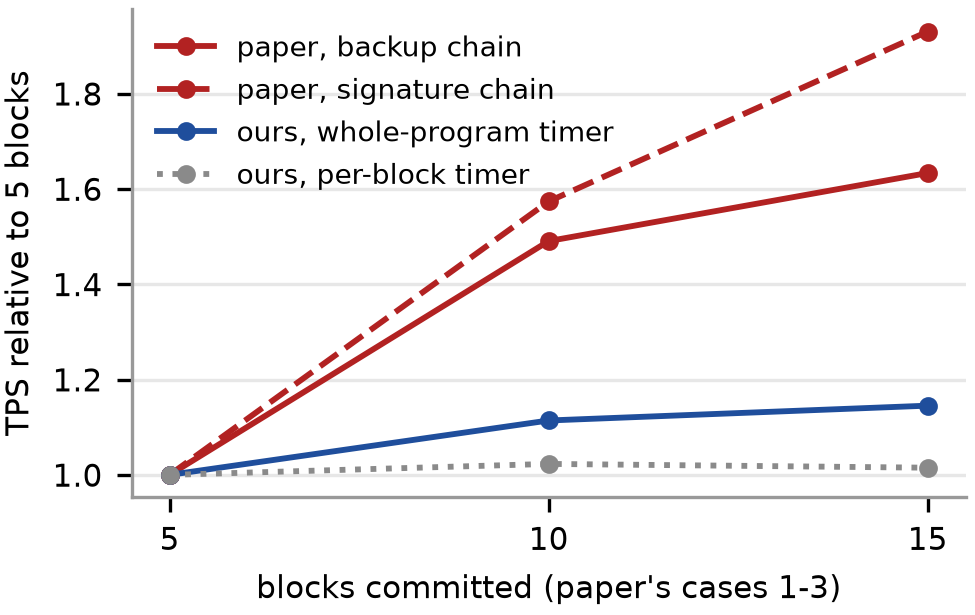
\includegraphics[width=\columnwidth]{figs/r_tps.png}
\caption{TPS relative to the 5-block case. The paper's TPS rises; ours rises too once the timer
covers the whole program, and stays flat with a per-block timer.}
\label{fig:tps}
\end{figure}

If a run costs a fixed setup time $F$ plus $p$ seconds per block, TPS improves with more blocks
because $F$ is spread over more transactions (\emph{amortisation}), like a taxi's fixed fee. We
fitted the paper's own timings to $F + p \times \text{blocks}$. The fit is almost exact
($R^2 = 0.989$ and $0.9999$): $F = 1.72$\,s and $p = 0.261$\,s on the backup chain, so setup is
55\% of the 5-block run (72\% on the signature chain). With $r = F/p$, the predicted TPS ratio
between 15 and 5 blocks is $3(r+5)/(r+15)$: 1.61 and 1.93 for the two chains, against the paper's
1.63 and 1.93. We then timed our build around the whole program, starting a new process each
time. Our TPS rose too, from 771 to 883 (Figure~\ref{fig:tps}), matching the predicted 1.14.
\textbf{Observation:} the paper's TPS gain is not consensus becoming faster. Per block nothing
changes, and TPS levels off near 383 (backup chain) and 417 (signature chain). With only three
points per chain, this is a strong explanation rather than a proof.

\subsection{B: A fair model comparison}
BitcoinHeist mixes very different scales: \texttt{income} is in satoshi and reaches about
$5\times10^{13}$, while other features are small counts or fractions. KNN classifies by distance,
so on raw values it effectively compares income alone. We log-transformed and standardised the
features, fitting the scaler on training data only to avoid \emph{data leakage}. On the paper's
data (5 seeds), KNN's balanced accuracy rose from 0.52 to 0.73, and its accuracy (93.6\%) moved
ahead of the decision tree (91.8\%). Logistic regression stayed at 0.50 and still flagged 99.7\%
of benign rows: its problem is its straight-line decision boundary, not scaling, which corrects
our mid-semester explanation. The tree models did not change, as expected. At natural balance,
weighting the rare class helped the random forest slightly (F1 0.26 to 0.36), while scaling made
KNN worse (F1 0.22 to 0.15), which we cannot explain.

\subsection{C: The detector learns the year}
\label{sec:c}

\begin{figure}[t]
\centering
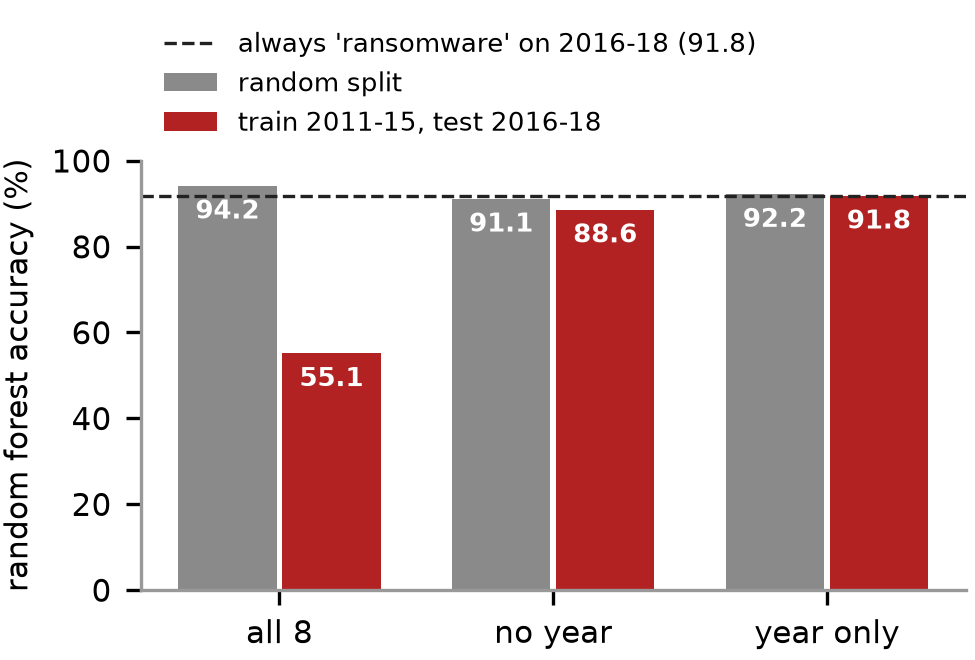
\includegraphics[width=\columnwidth]{figs/r_year.png}
\caption{Random forest accuracy on the paper's data with a random split versus a temporal split,
for three feature sets.}
\label{fig:year}
\end{figure}

Every BitcoinHeist row has a year, and ransomware is concentrated in a few: 2016 alone holds
37.7\% of all ransomware rows and 2014 holds 24.9\%. A model can therefore score well by learning
which years were suspicious, a form of \emph{shortcut learning} \citep{geirhos2020shortcut}. A
random split, as used by the paper and by our mid-semester work, places every year in both training
and test, so the shortcut works. A real detector is trained on the past and used on the future,
so we used a \emph{temporal split} \citep{pendlebury2019tesseract}: train on 2011--2015, test on
2016--2018 (5 seeds, same 90/10 data).

Accuracy fell from \textbf{94.2\% to 55.1\%} (balanced accuracy 0.52), well below the 91.8\% that
always answering ``ransomware'' scores on those years (Figure~\ref{fig:year}). The decision tree
fell to 48.7\%. On the random split, the year column alone scored 92.2\%, more than all seven
features that describe the address's behaviour (91.1\%). Removing the year did not fix the
future-years result: 88.6\% accuracy but 0.57 balanced accuracy, flagging 80\% of benign rows. A
second cut (train up to 2016) agreed: 60.8\% against a 75.8\% baseline. \textbf{Observation:} the
high accuracy on BitcoinHeist, ours and the paper's, comes largely from a calendar shortcut. This
corrects our mid-semester report, which concluded that the year was useful signal because removing
it lowered accuracy on a random split.

\subsection{E: Retraining every year does not help}

\begin{figure}[t]
\centering
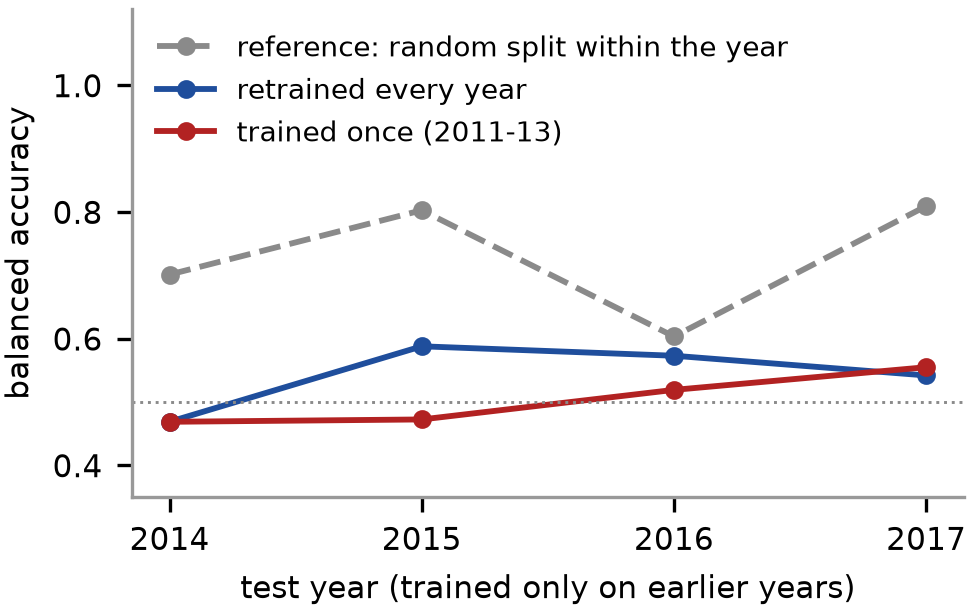
\includegraphics[width=\columnwidth]{figs/r_retrain.png}
\caption{Balanced accuracy on each year, using only earlier years for training (no year feature).}
\label{fig:retrain}
\end{figure}

A hospital would retrain its model as new data arrives, so for each year from 2014 to 2017 we
trained on all earlier years and tested on that year. Retrained yearly, balanced accuracy was
0.47--0.59, close to guessing, with about 80\% of benign rows flagged (Figure~\ref{fig:retrain}).
Training only on the last two years was no better. The dataset labels each ransomware row with its
family (for example CryptoWall, Locky or Cerber), so we also measured how much of each year came
from families never seen before: 89\% in 2014, 2\% in 2015, 98\% in 2016 and 1\% in 2017. In 2015
and 2017, almost every ransomware row belonged to a family the model had trained on a year earlier,
and the model still scored near 0.5. \textbf{Observation:} the failure is not only new families.
The same family produces different address statistics a year later (\emph{concept drift}), so
these eight features cannot carry a detector forward in time.

\subsection{D: The poisoning alarm}
\label{sec:d}
Our drift alarm scores each incoming honeypot batch by its \emph{Mahalanobis distance}
\citep{mahalanobis1936} from past data, and raises an alarm above a threshold, before the batch is
committed permanently to \sigrw{}. At mid-semester the threshold (3.0) was chosen before
measuring. We scored 30 poisoned batches per setting (three attacks, three poisoning budgets) and
300 clean batches of each kind. The highest score of any batch was 0.52, so the alarm \textbf{could
never fire}. With a threshold set from data, allowing 5\% false alarms on normal batches, label
flipping and feature poisoning were flagged 100\% of the time. A batch of genuine ransomware with
no poison, an honest outbreak, was flagged 99--100\% of the time as well. \emph{Anchor-point}
poisoning, which places fake samples at the centre of the data, scored lower than every clean batch;
an alarm that also fires on unusually low scores (2.5\% false alarms in each direction) caught it
in every case. \textbf{Observation:} the
alarm reacts to one-sided batches, not to poison, so during a real outbreak it would block exactly
the data the detector needs.

\subsection{F: One server holds every backup key}

\begin{figure}[t]
\centering
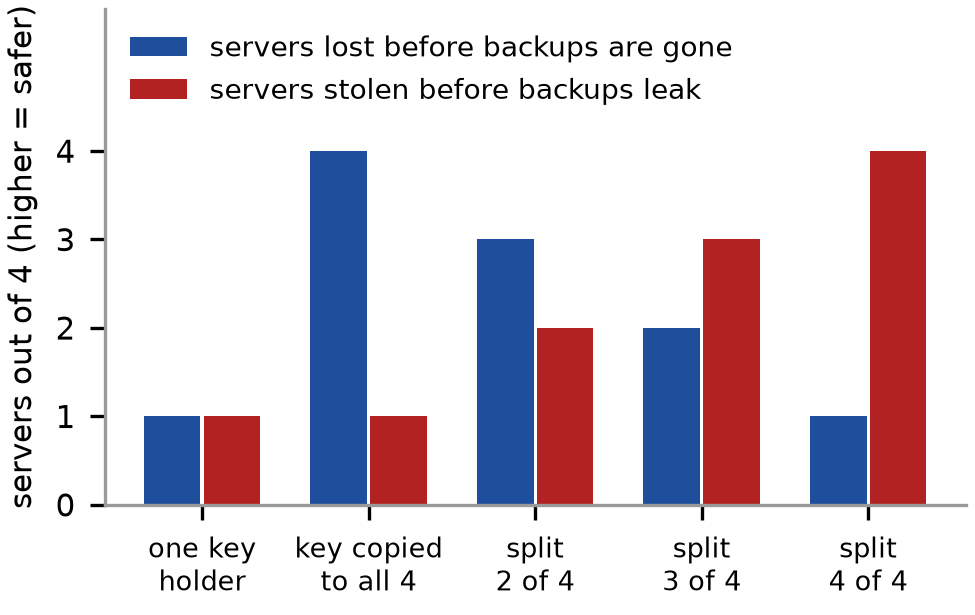
\includegraphics[width=\columnwidth]{figs/r_keys.png}
\caption{How many of the four servers must be lost or stolen before backups are lost or leak,
for each way of holding the key. All 16 combinations were tested.}
\label{fig:keys}
\end{figure}

In the paper, each backup is encrypted to the public key of the server that collected it. The chain
copies the encrypted backup to all four servers, but only that one server can decrypt it: four
copies of the locked box, one key. We showed both failures on our real pipeline. With the key
holder removed, \textbf{0 of 4} hospital systems could be recovered, although all four chain
replicas were intact. With its private key stolen, an attacker read \textbf{4 of 4} systems'
backups from another server's replica. The key holder is a \emph{single point of failure}, and an
obvious target for the ransomware itself.

Our repair uses \emph{Shamir secret sharing} \citep{shamir1979share}. Each backup's AES key is split
into four shares, one wrapped to each server, such that any two rebuild the key and one share alone
reveals nothing. We tried all 16 combinations of lost and stolen servers
(Figure~\ref{fig:keys}). With 2-of-4 sharing, backups are lost only if 3 servers go down and leak
only if 2 are stolen, compared with 1 and 1 before. If each server independently fails with
probability 0.1, the chance of losing the backups drops from 10\% to 0.37\%, and of a leak from
10\% to 5.2\%. Copying the key to every server would be the wrong fix: any single stolen server
would then leak everything. Sealing a 4\,KB backup piece took 0.54\,ms instead of 0.12\,ms, and each
transaction carries about 400 extra bytes.

\subsection{G: Slow ransomware poisons the backups}

\begin{figure}[t]
\centering
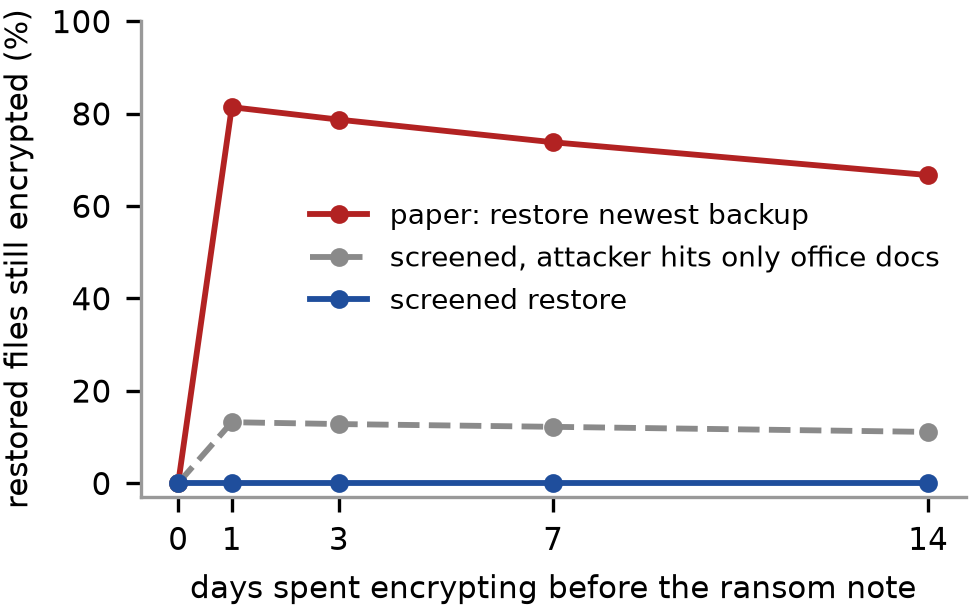
\includegraphics[width=\columnwidth]{figs/r_slowburn.png}
\caption{Share of restored files that are still encrypted, against the number of days the
ransomware spends encrypting (10 runs per point).}
\label{fig:slowburn}
\end{figure}

Alg.~5 restores the newest backup. That works only if ransomware encrypts everything at once,
after the last backup. Real ransomware often encrypts gradually over days
(\emph{slow-burn}), and every nightly backup in that period saves the encrypted files. Because the
chain is immutable, it then preserves the ransomware's output as faithfully as real data. For
safety, all files in this experiment are synthetic and kept in memory, and encryption is modelled
by overwriting bytes with random bytes, which is what encrypted data looks like statistically.

On our real pipeline, with daily backups through pBFT and an attack that encrypted files over 7
days, Alg.~5 restored the day-16 backup and \textbf{all 16 encrypted files came back encrypted}.
Every integrity check passed, including the hospital system's own signature on its backup, because
the infected system really did send those bytes. The chain guarantees \emph{integrity}, not that
the data is good. Across 10 simulated runs, one day of slow encryption already left 81\% of
restored files encrypted (Figure~\ref{fig:slowburn}); only an attack that encrypts everything after
the last backup is handled.

\begin{table}[t]
\centering
\small
\begin{tabular}{@{}lcccc@{}}
\toprule
\textbf{Check level} & \textbf{FA} & \textbf{Full} & \textbf{Header} & \textbf{Stripes} \\
\midrule
randomness only & 100\% & yes & no & no \\
+ file format & 0\% & yes & yes & text, scans \\
+ write-once images & 0\% & yes & yes & all but office \\
\bottomrule
\end{tabular}
\caption{Backup screening against three encryption styles: whole file, first 4\,KB only, and thin
stripes that keep the header. FA: false alarms on clean photos and office documents.}
\label{tab:screen}
\end{table}

\paragraph{The fix: screening backup contents.} We added a check that looks inside each backup. It
runs on the cloud server, which sees the backup before encrypting it, never on the infected
machine. A naive check that flags random-looking data (high \emph{entropy}) is useless: photos and
office documents are already compressed, look random, and are all flagged
(Table~\ref{tab:screen}). Our check instead uses file type. File headers (\emph{magic bytes}) must be
intact, text files must still be valid text, scan images must contain no random-looking patches,
and medical images, which are write-once, must match their first version on the chain. This
catches full and header-only encryption, and \emph{intermittent} encryption of images and text.
At restore time, Alg.~5 restores the newest backup that passes. In the 7-day attack this gave
\textbf{0\%} encrypted files, at the cost of rolling back 7 days of work. Run at backup time, the
check doubles as an early alarm: it fired on the attack's first day, and only 7 of 48 files were
encrypted before isolation (instead of 48). \textbf{Remaining gap:} office documents are both
compressed and legitimately edited, so neither rule applies. An attacker who encrypts only those,
in thin stripes with the header intact, passes every check, leaving about 12\% of files encrypted.

\begin{table}[t]
\centering
\small
\begin{tabular}{@{}p{1.55cm}p{3.6cm}p{1.45cm}@{}}
\toprule
\textbf{Area} & \textbf{Outcome} & \textbf{Status} \\
\midrule
A timing & setup cost averaged out; TPS levels off near 400 & explained \\
B models & KNN 0.52 $\to$ 0.73; LR unchanged & partly fixed \\
C, E detection & near guessing on unseen years, retrained or not & broken \\
D alarm & flags real outbreaks as poison & limited \\
F keys & 2-of-4 shares: 3 lost or 2 stolen needed & repaired \\
G recovery & screening restores clean data; striped office files pass & repaired, one gap \\
\bottomrule
\end{tabular}
\caption{Summary of the work after mid-semester.}
\label{tab:summary}
\end{table}

% =====================================================================================
\section{Discussion}
\label{sec:discussion}

\paragraph{Limitations of the paper.} Putting both halves of the project together, we found the
following problems with BSFR-SH (Table~\ref{tab:summary} summarises the post-mid-semester part):
\begin{itemize}
\setlength\itemsep{0pt}
\item \textbf{Evaluation.} The 98.98\% comes from a 46,014-row sample that is 90\% ransomware,
where a constant answer scores 90\%. No hyperparameters, seed or split method are given, and the
result did not reproduce (94.4\%).
\item \textbf{Shortcut and drift.} On a random split the detector learns the calendar; on future
years it is near guessing, and retraining does not help (\S\ref{sec:c}). This is a common pitfall
in security ML \citep{arp2022dos}.
\item \textbf{Mismatch.} The framework detects running ransomware from honeypot behaviour, but the
paper evaluates on Bitcoin payment records, a different problem.
\item \textbf{Consensus bound.} The 51\% argument does not apply to pBFT; two of four servers fork
the chain, and one malicious plus one slow server stalls it.
\item \textbf{Throughput.} The rising TPS is amortised setup cost, not scalability.
\item \textbf{Preprocessing.} ``Remove the abnormalities'', read literally, deletes the ransomware
class.
\item \textbf{Recovery.} One server holds every backup key, and restoring the newest backup returns
slow ransomware's output. Immutability protects backups from tampering, not from being bad when
written.
\item \textbf{Case~3.} Automating ransom payment is unsafe: the paper itself notes there is no
guarantee the key arrives.
\end{itemize}

\paragraph{What the paper gets right.} The two-chain design is sound: detection data and recovery
data never share servers or state, so compromising one does not compromise the other. pBFT is the
right consensus choice over Raft for this setting. The session protocol is secure. Using an
immutable ledger to protect a detector's training data is a sensible idea, provided the data is
checked before it is written.

% =====================================================================================
\section{Conclusion}
We rebuilt BSFR-SH completely and tested its claims. Its detection result does not reproduce,
rests on a test set where a constant answer scores 90\%, and mostly reflects which years had
ransomware. Its consensus layer is weaker than claimed, and its throughput curve is an artefact of
timing. After mid-semester we also attacked its recovery step, the part a hospital relies on most,
and found two serious gaps, a single key holder and slow-burn ransomware, each of which we
repaired and measured: 2-of-4 key sharing, and backup screening that also gives an early alarm.
The architecture is worth building on, but the published numbers and the informal security
argument should not be relied on as they stand.

% =====================================================================================
\section*{Limitations}
Our own work has the following limitations.
\textbf{Synthetic honeypot data.} The honeypot features are generated statistically, not collected
from real ransomware. The detector trained on them does not transfer to real malware datasets
(0.50 balanced accuracy), so the honeypot results show how the pipeline behaves, not real-world
detection rates.
\textbf{Unexplained reproduction gap.} After eight hypotheses, 1.51 points of the gap to 98.98\%
remain unexplained, partly because the paper gives no hyperparameters or split method.
\textbf{Small timing fit.} The amortisation explanation (A) rests on three points per chain, and we
do not know exactly what the paper's timer included. Our timings come from a single machine and
are not comparable in absolute terms.
\textbf{Simulated slow-burn attack.} Experiment G uses synthetic files and models encryption as
random bytes. The 0\% false-alarm rate of screening is therefore optimistic: real scans sometimes
receive header corrections, some medical images are stored compressed, and file types come from
extensions that an attacker could change. The early-alarm result assumes isolation stops the
ransomware as soon as the alarm fires.
\textbf{Prototype repairs.} The key-sharing scheme (F) is implemented and tested as a separate
cryptographic module but is not switched on in the backup pipeline, and it does not support share
refresh or detect which server supplied a bad share. The screening check is opt-in.
\textbf{Untested follow-ups.} We did not test an attacker who adds noise to anchor-point poison to
avoid the two-sided alarm, and we could not explain why scaling hurts KNN at natural class
balance.
\textbf{Scope.} We study one paper's design. Data theft before encryption (double extortion),
insider attacks on server registration, and network-level timing are outside what we tested.

\section*{Ethics Statement}
No real malware was written, downloaded or executed. Honeypot samples are statistical feature
vectors, slow-burn encryption is simulated in memory, and the paper's ransom-payment step is a
simulated decision that is always blocked and cannot contact any network or wallet. BitcoinHeist is
a public dataset of Bitcoin addresses.

\bibliography{references}

\end{document}
